\documentclass[handout]{beamer}

\usepackage[utf8]{inputenc} % Language and font encoding
\usepackage[icelandic]{babel}
\usepackage[T1]{fontenc}


\usepackage{tikz}
\usepackage[listings,theorems]{tcolorbox}
\usepackage{booktabs}
\usepackage{minted} %Minted and configuration
\usemintedstyle{default}

\renewcommand{\theFancyVerbLine}{\sffamily \arabic{FancyVerbLine}}
%%%%%%%%%%%
% More math
%%%%%%%%%%%
\newcommand{\Mod}[1]{\ \text{mod}\ #1}

%%%%%%%%%%%%%%%%%%%%%%
% Beamer configuration
%%%%%%%%%%%%%%%%%%%%%%
\setbeamertemplate{navigation symbols}{}
\usecolortheme{dove}
\setbeamercolor{frametitle}{fg=white}

\usebackgroundtemplate%
{%
\vbox to \paperheight{

\includegraphics[width=\paperwidth]{Pics/hi-slide-head-2016}

\vfill
\hspace{0.5cm}
\includegraphics[width=0.3\paperwidth]{Pics/hi-von-logo}
\vspace{0.4cm}
    }%
}

\AtBeginSection[]
{
  \begin{frame}<beamer>
    \frametitle{Yfirlit}
    \tableofcontents[currentsection]
  \end{frame}
}

\setbeamerfont{frametitle}{size=\normalsize}
\addtobeamertemplate{frametitle}{}{\vspace*{0.5cm}}

%%%%%%%%%%%%%%%%%%%%%%%%%
% tcolorbox configuration
%%%%%%%%%%%%%%%%%%%%%%%%%

% Setup from: http://tex.stackexchange.com/a/43329/21638
\tcbset{%
    noparskip,
    colback=gray!10, %background color of the box
    colframe=gray!40, %color of frame and title background
    coltext=black, %color of body text
    coltitle=black, %color of title text 
    fonttitle=\bfseries,
    alerted/.style={coltitle=red, colframe=gray!40},
    example/.style={coltitle=black, colframe=green!20, colback=green!5},
}


%%%%%%%%%%%%%%%%%%%%%%%
% Further configuration
%%%%%%%%%%%%%%%%%%%%%%%
\hypersetup{colorlinks=true,pdfauthor={Eirikur Ernir Thorsteinsson},linkcolor=blue,urlcolor=blue}
\graphicspath{{./Pics/}}

\author{Eiríkur Ernir Þorsteinsson}
\institute{Háskóli Íslands}
\date{Haust 2016}

\title{Stærðfræðimynstur í tölvunarfræði}
\subtitle{Vika 12, fyrri fyrirlestur}

\begin{document}

\begin{frame}
\titlepage
\end{frame}


\section{Inngangur}

\begin{frame}{Í síðasta tíma}
\begin{itemize}
 \item Euler-vegir
 \item Hamilton-vegir
 \item Leit að stystu vegum
\end{itemize}
\end{frame}

\section{Lagnet}

\begin{frame}{Lagnet}
\begin{tcolorbox}[title=Lagnet]
Net er kallað lagnet (e. \emph{planar graph}) sé hægt að teikna það í sléttan flöt þannig að hnútar séu punktar og leggirnir samfelldir einfaldir ferlar sem skerast aldrei nema í endapunktunum. Slík teikning er kölluð sléttunet (e. \emph{planar representation}).
\end{tcolorbox}
\end{frame}

\begin{frame}{Dæmi}
\begin{center}
Netið $K_4$ er lagnet.

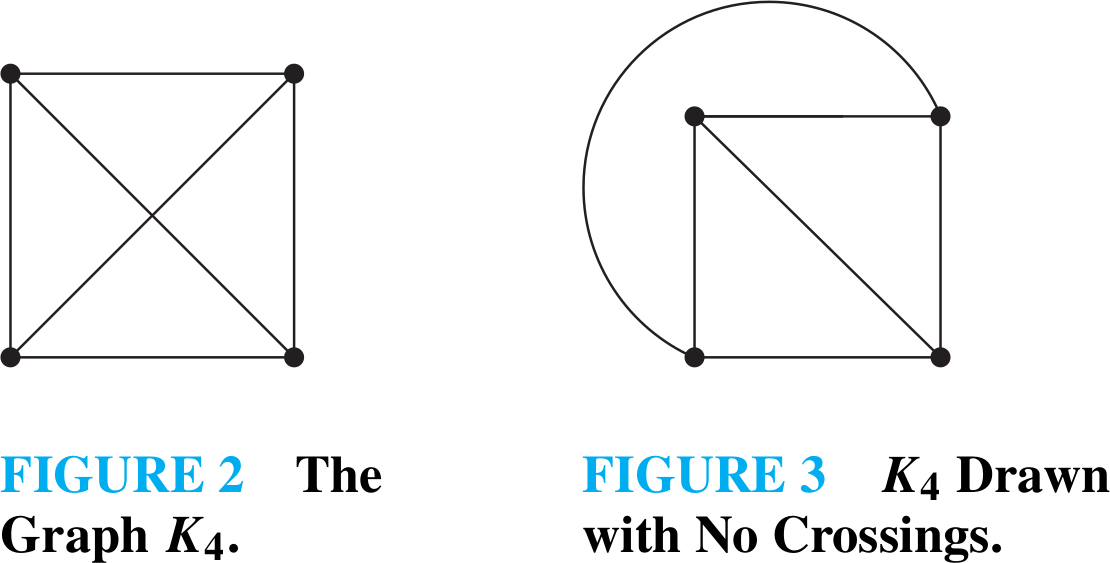
\includegraphics[width=0.8\textwidth]{graph-planar-k4}
\end{center}
\end{frame}

\begin{frame}{Dæmi}
\begin{center}
Netið $Q_3$ er lagnet.

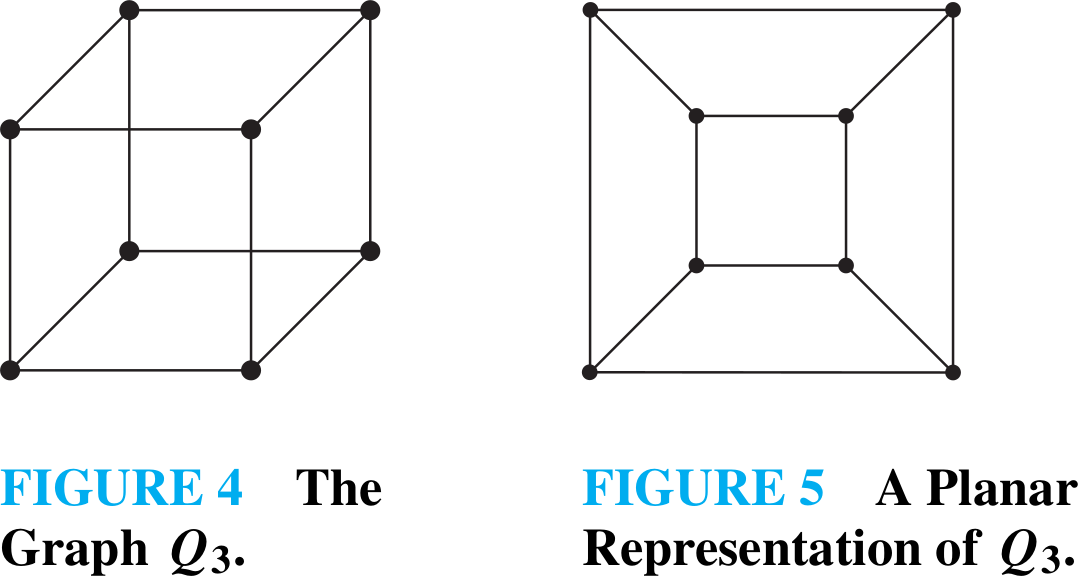
\includegraphics[width=0.8\textwidth]{graph-planar-q3}
\end{center}
\end{frame}

\begin{frame}{Dæmi}
\begin{center}
Netið $Q_{3,3}$ er ekki lagnet.

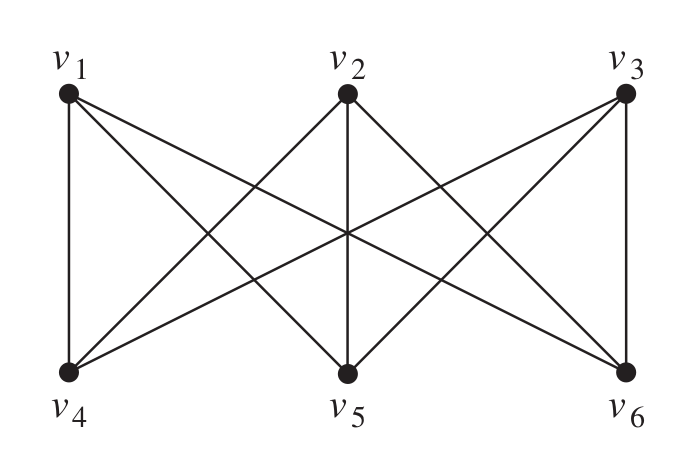
\includegraphics[width=0.8\textwidth]{graph-nonplanar-k33}
\end{center}
\end{frame}

\section{Möskvar}

\begin{frame}{Möskvar}
\begin{columns}
\column{0.5\textwidth}
Sléttuneti má skipta upp í svæði sem kallast möskvar (e. \emph{regions}). Einn möskvinn er ótakmarkað svæði, hinir afmarkast af leggjum netsins.
\column{0.5\textwidth}
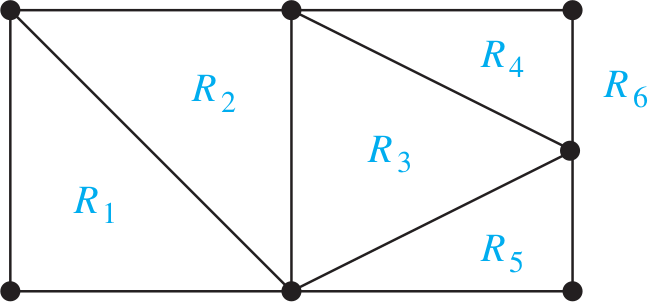
\includegraphics[width=\linewidth]{graph-regions}

Hér eru möskvar netsins merktir með $R_i$.
\end{columns}
\end{frame}

\begin{frame}{Jafna}
\begin{tcolorbox}[title=Jafna Eulers]
Látum $G$ vera einfalt samanhangandi lagnet með $e$ leggjum, $v$ hnútum og $r$ möskvum. Þá er

\[
 r = e - v + 2.
\]

\end{tcolorbox}
\end{frame}

\begin{frame}{Dæmi}
Hversu marga möskva hefur sléttunet með 20 hnútum sem allir eru af stigi 3?
\pause

\vspace{1cm}
Hér er $v=20$. Summa stiganna er $3v = 60 = 2e$, svo $e = 30$. Þá gefur jafna Eulers:

\[
 r = e - v + 2 = 30 - 20 + 2 = 12
\]

\end{frame}

\begin{frame}{Fylgisetningar}
Eftirfarandi fylgisetningar eiga við einfalt samanhangandi lagnet $G$ með $v$ hnúta og $e$ leggi:
\begin{tcolorbox}
Sé $v \geq 3$, þá er $e \leq 3v - 6$.
\end{tcolorbox}

\begin{tcolorbox}
$G$ hefur hnút af stigi sem er ekki hærra en $5$.
\end{tcolorbox}

\begin{tcolorbox}
Hafi $G$ engar rásir af lengd 3 og $v \geq 3$, þá er $e \leq 2v -4$
\end{tcolorbox}
\end{frame}

\begin{frame}{Dæmi}
Notum síðustu fylgisetninguna til að sýna að $K_{3,3}$ sé ekki lagnet. \pause

\vspace{1cm}
$K_{3,3}$ hefur meira en 3 hnúta og hefur engar rásir af lengd $2$ þar sem það er tvíhlutanet, svo setningin gildir.

Netið hefur 6 hnúta og 9 leggi. En við sjáum að $9 \geq 2v - 4 = 8$, svo $K_{3, 3}$ getur ekki verið lagnet.
\end{frame}

\section{Grannmótanir}

\begin{frame}{Grannmótun}
Tvö net eru grannmóta (e. \emph{homeomorphic}) sé hægt að mynda þau úr sama neti með uppskiptingum á leggjum:
\begin{center}
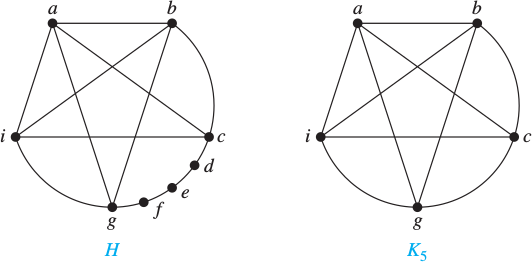
\includegraphics[width=0.8\textwidth]{graph-homeomorphism}
\end{center}
\end{frame}

\begin{frame}{Setning Kuratowskis}
\begin{tcolorbox}[title=Setning Kuratowskis]
Net $G$ er lagnet þá og því aðeins að það innihaldi ekkert hlutnet sem er grannmóta $K_5$ eða $K_{3,3}$.
\end{tcolorbox}

\end{frame}


\section{Hnútalitun}

\begin{frame}{Hnútalitun}
\begin{tcolorbox}[title=Litun]
Litun (e. \emph{coloring}) á einföldu neti er ákvörðun á litum á hverjum hnút netsins svo að engir tveir aðlægir hnútar hafi sama lit.
\end{tcolorbox}

\begin{tcolorbox}[title=Litunartala]
Litunartala nets $G$ er minnsti fjöldi lita sem þarf til að lita hnúta netsins. Litunartala $G$ er táknuð með $\chi(G)$.
\end{tcolorbox}

\end{frame}

\begin{frame}{Fjögurra lita setningin}
\begin{tcolorbox}[title=Fjögurra lita setningin]
Litunartala lagnets er 4.
\end{tcolorbox}
Setningin var upphaflega sett fram sem tilgáta um miðja 19. öld. Hún var sönnuð árið 1976, þá með aðstoð tölvu.
\end{frame}

\begin{frame}{Hagnýtingar}
\begin{itemize}
 \item Hnútalitanir má hagnýta á ýmsa vegu
 \begin{itemize}
  \item Litum landakort
  \begin{itemize}
   \item Lönd eru hnútar, landamæri eru leggir
  \end{itemize}
  \item Ákvörðum tímasetningar fyrir lokapróf
  \begin{itemize}
   \item Táknum námskeið með hnútum, leggur á milli sé nemandi í þeim báðum
   \item Hver möguleg tímasetning fyrir próf er einn litur
  \end{itemize}
 \end{itemize}
 \item Hnútalitunarvandamálið er þekkt NP-complete vandamál
\end{itemize}

\end{frame}


\begin{frame}{Næst}
Kafli 11.1 (kynning á trjám), kafli 11.2 (hagnýtingar á trjám), e.t.v. kafli 11.3 (ferðast eftir trjám)
\end{frame}


\end{document}
